\chapter{Final results and summary discussion}\label{ch:final-results-and-summary-discussion}


\section{Results}\label{sec:results}

Presented model was trained and tested using various parameters.
The changes were affected by the input data as well as the neural network parameters.
The final dataset properties used to train the presented model are described in \mbox{Tab.~\ref{tab:dataset}}.
The input picture size was forced by the used transfer learning model.
This limitation had an effect on resizing original pictures of sequences to the required one by the used neural network.

\begin{table}[!hbt]
    \centering
    \begin{minipage}{.49\textwidth}
        \centering
        \captionsetup{width=\linewidth}
        \captionof{table}{Dataset properties} \label{tab:dataset}
        \begin{tabular}{p{0.6\textwidth}p{0.29\textwidth}}
            \hline
            Users                    & 46                 \\ \hline
            Human users              & 45                 \\ \hline
            Bot users                & 1                  \\ \hline
            Sequences                & 639                \\ \hline
            Minimal sequence length  & 50                 \\ \hline
            Model input picture size & 299 x 299 {[}px{]} \\ \hline
        \end{tabular}
    \end{minipage}
    \hfill
    \begin{minipage}{.5\textwidth}
        \centering
        \captionsetup{width=\linewidth}
        \captionof{table}{Confusion matrix values} \label{tab:confusion-matrix}
        \begin{tabular}{p{0.50\textwidth}p{0.12\textwidth}}
            \hline
            False negatives       & 19    \\ \hline
            False positives       & 0     \\ \hline
            True negatives        & 327   \\ \hline
            True positives        & 0     \\ \hline
            False rejection rate  & 100\% \\ \hline
            False acceptance rate & 0\%   \\ \hline
        \end{tabular}
    \end{minipage}
\end{table}

The total amount of sequences depends on the minimal sequence length, because sequences that were shorter than 50 were simply rejected.
The sequence split point was established by the time interval between two consecutive actions and in presented work was fixed to 1 second.
The minimal sequence length was fixed based on several attempts.
Shorter sequences than the determined ones resulted in apparently lower accuracy, when longer ones did not improve performance at all.
The length of 50 seemed to be the golden mean between accuracy and amount of sequences.

The charts presented in \mbox{Fig.~\ref{fig:accuracy} and Fig.~\ref{fig:loss}} show that the model accuracy reaches the level of 94\% with 69.5\% value of the loss function.
It can be seen that the model accuracy during the testing part is in most epochs higher than the one in the training phase.
It is caused by an imbalanced dataset which was the input for the presented model, where
the amount of user data for testing was greater than the one generated by a bot.
It is the direct effect of having more user data in the whole dataset.
The impact is also seen on the loss function chart \mbox{(Fig.~\ref{fig:loss})}, where values are lower in the testing part.

\begin{figure}[!hbt]
    \centering
    \begin{minipage}{.5\textwidth}
        \centering
        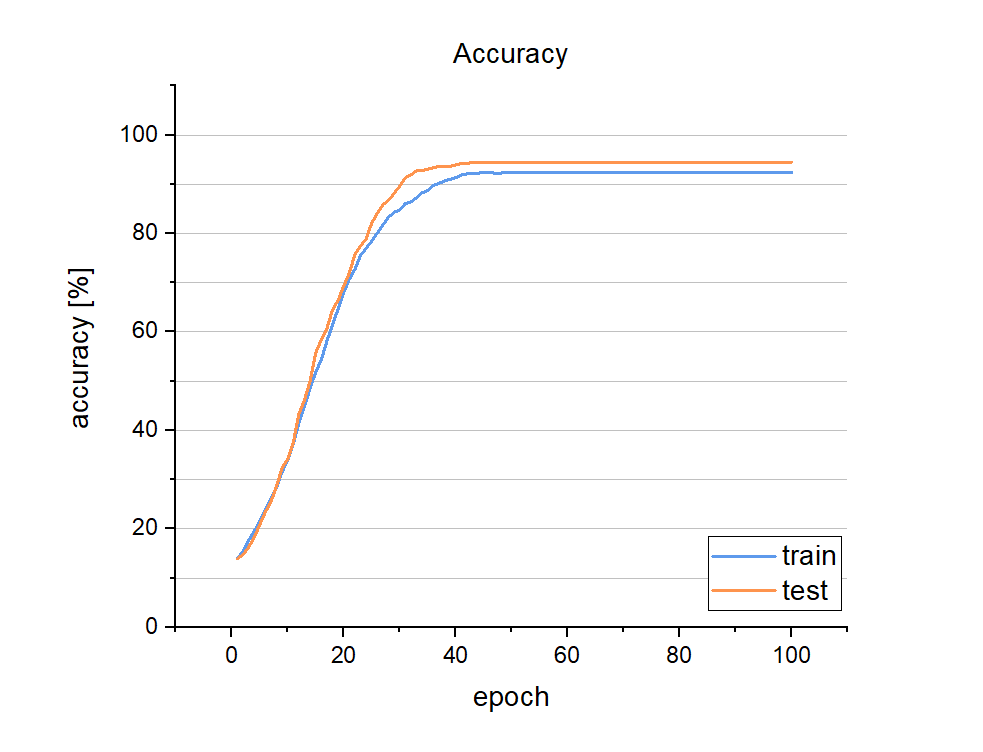
\includegraphics[width=\linewidth]{resources/accuracy.png}
        \captionsetup{width=\linewidth}
        \captionof{figure}{Accuracy of presented model}
        \label{fig:accuracy}
    \end{minipage}%
    \begin{minipage}{.5\textwidth}
        \centering
        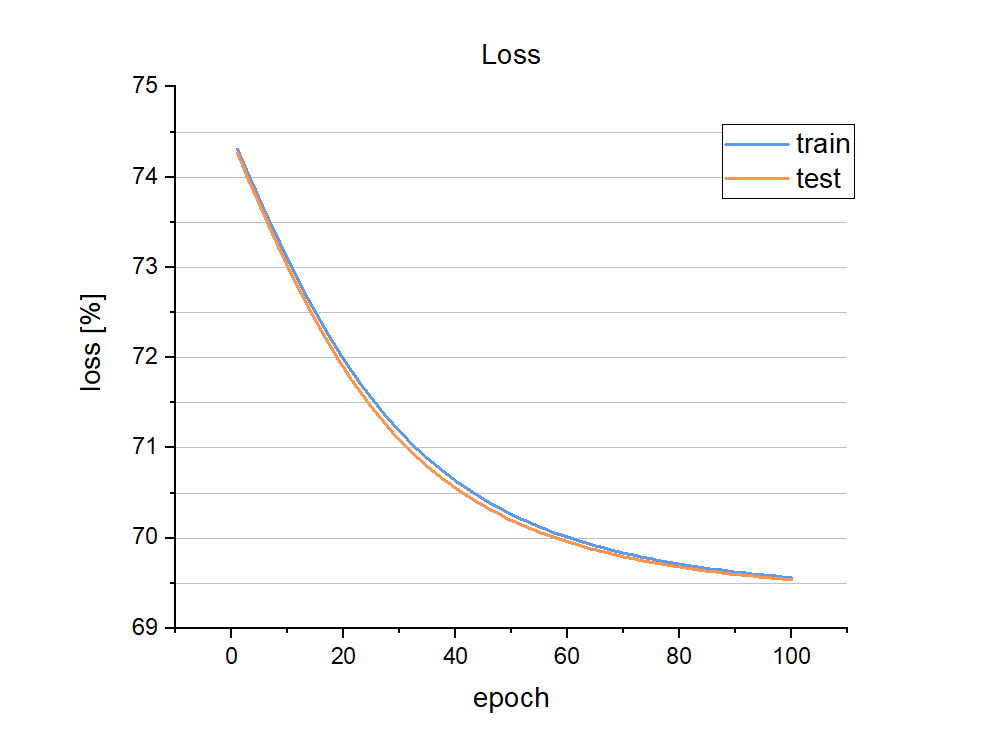
\includegraphics[width=\linewidth]{resources/loss.png}
        \captionsetup{width=\linewidth}
        \captionof{figure}{Value of loss function used in model}
        \label{fig:loss}
    \end{minipage}
\end{figure}

Moreover, due to the low amount of data, the model had some problems with prediction.
At the beginning of the learning procedure, user and bot data were treated with equal importance.
With the successive epochs, user data outshone bot dataset.
It can be seen \mbox{(Tab.~\ref{tab:confusion-matrix})} that after the learning process, there were no true positives, which suggests that the model learned only one type of data.
The model always predicted that the input data was the user's one.
It is the result of a large amount of user data in comparison to bot sequences, whereas it is not the result of having only one bot user and many human users, because each user's sequence was joined into a global one.

Chong et al.~\cite{Main} present similar approach to related problem, but the results achieved in this study show that the presented solution behaves unilaterally.
In many cases from cited work, authors achieved very low values of \gls{frr} and \gls{far}.
In this work, using \gls{cnn}'s as a core of a solution, totally different results were achieved.
The authors of this study consider the imbalanced dataset as the main foundation of that unexpected behavior.
Despite the numerous efforts taken, the results are unsatisfactory.
The obtained accuracy chart (Fig.~\ref{fig:accuracy}) is somehow expected due to the dominance of one kind of data in the binary selection problem.
However, the loss function (Fig.~\ref{fig:loss}) as well as confusion matrix (Tab.~\ref{tab:confusion-matrix}) have undesirable values.


\section{Limitations, conditions and problems}\label{sec:limitations-conditions-problems}
Although the model was considered using different sets of parameters and various approaches, it did not perform well.
Due to certain limitations, some aspects of the model performance could not have been improved.
Some problems that have a great impact on the overall results are described in the following sections.

\subsection{Dataset limitation}\label{subsec:dataset-limitation}
The main reason for poor performance has to be an insufficient dataset used in the study.
The search for proper and publicly available data resulted in failure.
In other related works, like Chong et al.~\cite{Main} or Antal et al.~\cite{antal2019intrusion} points at the Balabit Mouse Challenge Dataset as the most popular and comprehensive, yet still quite small data source for mouse sequences and behaviors.
However, this dataset is not appropriate for the problem considered in this study.

The Balabit dataset consists of user sessions recorded on the remote machine.
The data includes the timing and position of the mouse cursor of ten different users.
The split dataset represents training sessions and test sessions.

In the training sessions, one can find 65 legitimate sessions of various lengths, wherein total gives 2,253,871 rows of registered user mouse actions.
The test sessions consist of 1,611 shorter sequences, that in total have 2,357,714 recorded actions, where during the session execution of the legal user, the illegitimate action happens --- the session is taken over by another user.
Illegal sessions are the mix of two legitimate users, and when the model considers the example it should assume one user, that is then interrupted and replaced by another user somewhere between the session.

This data does not relate to the problem given in the scope of this work --- the model that can distinguish legitimate human user and non-human bot behavior is taken into consideration.
This particular case is derived from the general problem of distinguishing two or more users and represents a more specific case of using mouse behavioral biometrics.

\subsection{Custom dataset research participation limitation}\label{subsec:custom-dataset-research}
Since no public dataset is available, the goal of this work was to collect exclusive and dedicated data for purpose of the study.
The custom environment\upperref{itm:data-collection} created as a playground for research participants was designed to collect and record the mouse data, but it did not serve the responsiveness of a real commercial website, and therefore it may be causing some confusion among the subject users.
By that means, data collecting was in some kind suggestive and task-oriented.
Given factors could have a negative impact on the quality of the collected data.

The other thing is that participation in the study was completely voluntary and community-based.
The advertisement for the ongoing study was posted on a couple of Facebook groups, which was the most available and large user community base.
However, such an approach resulted in non-supervised data gathering, and therefore some user actions could not be assessed as properly executed and caused disturbances and noises in the set.

The research gathered 63 unique users.
Overall user mouse actions collected are equal to 334,184 rows.
The number of bot actions registered and collected is equal to only 24,791 rows.\\
Such an uneven ratio of the data made the dataset imbalanced, which resulted in the model making assumptions about every sequence biased towards the class of human users.
Training set contained about 269,231 bot and user sequences, whereas the test set contained 89,744 sequences --- even using transfer learning technique, the dataset was too small for efficient model training.

\subsection{Finance limitation}\label{subsec:finance-limitation}
Another problem encountered when preparing the thesis was the limit of the finance intended.\\
Because the research was planned to reach many different users it had to be deployed and hosted on trusted and reliable resources.

Cloud services are really convenient way to handle such a project --- the hosting, computation, and storage resources can be acquired on-demand, with no time and commitment.
In the variety of different cloud solutions, in this case, the Google Cloud Platform was selected and used.
However, the cost of this kind of resources is high enough to be a limitation for the work.

\subsection{Time limitation}\label{subsec:time-limitation}
Due to the time limitation, the duration of the period when the data was collected could not be extended to broader terms, thus the research and the voluntary participation in data collection were canceled during the further implementation of the project --- the bot detection part\upperref{itm:bot-detection}, where the machine learning model was in build.

\section{Conclusions and further study}\label{sec:conclusions-and-further-study}

\subsection{Summary}\label{subsec:summary}
During the work on the presented solution, the steps to limit the impact of the imbalanced dataset were taken.
As an example, linear interpolation was used by connecting the points in recorded sequences.
Each used sequence originally consisted of many single discrete points without any additional pieces of information.
Interpolation provided an order between discrete coordinates and allowed feeding the neural network with additional information.

Another considered approach was a manipulation of the input data size.
The user's sequences were limited to the number of total bot sequences.
This solution was aimed to balance the dataset at the cost of fewer data.
The results of this approach turned out insufficient.
Because of the total amount of bot sequences, the total size of the dataset drastically shrank, which resulted in a performance deterioration.
On the other hand, the duplication of the bot sequences was used.
The idea was similar to the one before, but instead of reducing, the number of bot samples was increased by using a single sample several times.
It resulted in an artificially balanced dataset.
However, this approach did not increase performance at all.

Manipulation of the distribution of labels between training and testing dataset was also considered.
It was done by performing either an equalization of the total number of both types in the testing dataset and the distribution of samples between both datasets.
The first solution did not affect model performance, but the second one slightly improved overall performance if the ratio was close to 50:50.
When the number of training samples was significantly greater than testing ones, the accuracy decreased due to a very small number of bot samples in testing dataset.

Yet another attempt to reduce the impact of the inappropriate dataset was changing the dataset itself.
The developed serializing tool made it possible to create a few datasets from recorded data with different minimal sequence length limits.
Using longer sequences meant that the overall number of them would be smaller.
The authors tested several ones and found out that the best performance was for a length equal to 50, as it was mentioned before.

All of the presented approaches tended to minimize the dataset problem.
Some of them slightly improved performance and those were considered in the final solution.
Despite the efforts and attempts for improving the model, the described problem significantly worsened the performance of the model.

\subsection{Further study}\label{subsec:further-study}
According to the described issues, the authors find further study mainly in the improvement of the dataset.
Some efforts may be taken to extend the size of the recorded data.
Firstly, recording sequences of a bigger group of users may be proposed as a solution, especially enlarge the bot users to prevent imbalance.
Such a solution should improve the overall performance of the model or at least suggest other problems related to the quality of the dataset.\\
If the quality of the recorded samples would be inappropriate, the collection module\upperref{itm:data-collection} should be reviewed and improved.
The main object of interest should be the method of gathering the samples.
Delays and synchronization that can disturb the reliability of the data may be considered as a major area of study.

The different approach that may be taken into consideration is another machine learning model.
In the presented solution, the focus was on the two-dimensional convolutional neural network, taking an example from related works like Chong et al.~\cite{Main} and Wei et al.~\cite{a-deep-learning-approach-to-web-bot-detection-using-mouse-behavioral-biometrics}.
The work~\cite{Main} also shows other solutions, especially recursive neural networks.
Those kinds of neural networks are very popular in problems where the order and time intervals between samples have natural interpretations.
The problem which is described in this work also has similar properties.

These two described areas of study are found by the authors as the major to improve performance and reliability.
To deliver a safe and reliable solution to the commercial market further study is necessary.
